\graphicspath{{content/3_results/figures}}
\section{Current Sensor}

\subsection{Simulation}

After running initial simulations, it was clear that the constant assumed in the design stage for the dominant capacitor $C_f$ was too high. The capacitor value was then experimentally
increased to 100nF where a satisfactory response which was reasonably below 250 mV (10-20\%) was obtained. This section details the rest of the results of these simulations.

\begin{figure}[h!]
   \centering
   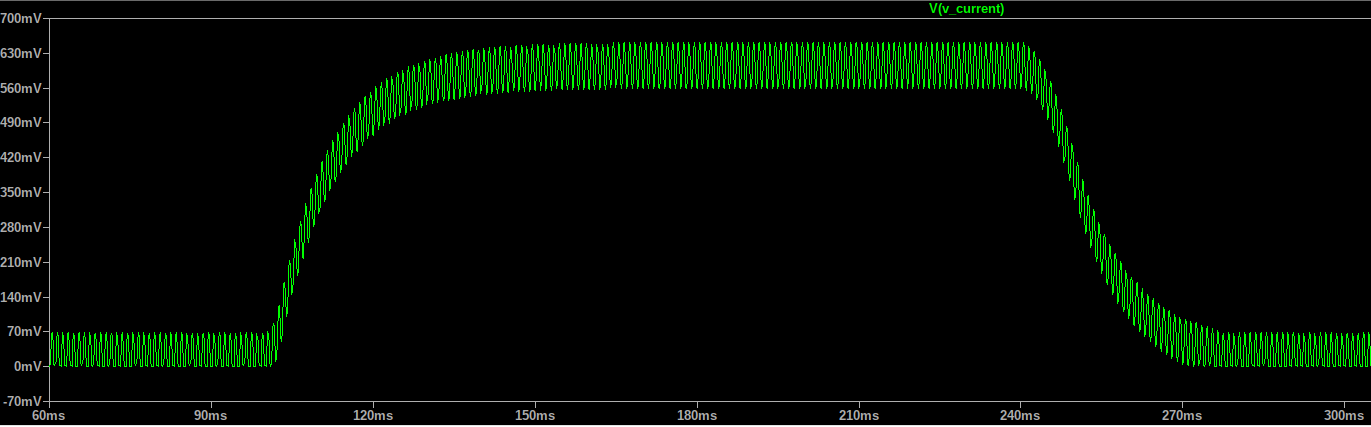
\includegraphics[width=.6\linewidth]{currentSensor_sim_stepResponse}
   \captionof{figure}{Output and Noise Level in Response to Step Input}
   \label{fig:simulation response}
\end{figure}

\begin{figure}[h!]
   \centering
   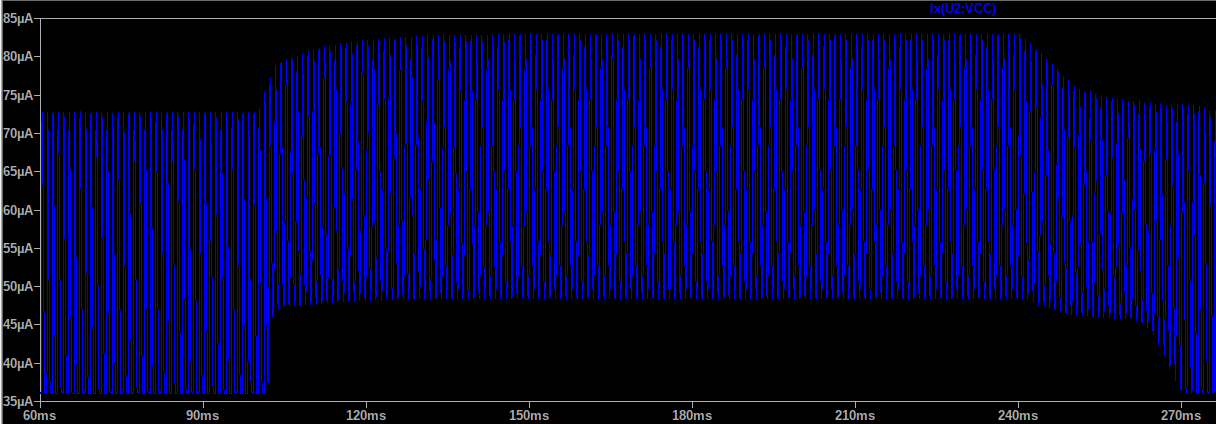
\includegraphics[width=.5\linewidth]{currentSensor_sim_currentDraw}
   \captionof{figure}{Current Draw}
   \label{fig:simulation_current}
\end{figure}

As can be seen, all specifications were adhered to:
\begin{itemize}
   \item The noise level at idle is well below the 250 mV requirement.
   \item The step response input changes 20-25 ms, which is below the 100 ms requirement.
   \item The power draw of the circuit (as measure at the positive terminal of the op-amp) is less than 85 uA, which is much less than the specified 150 uA.
\end{itemize}

Lastly, the input simulation parameters were modified during testing to analyze the various output voltages for different input currents. For input currents of 400mA, 500mA, 800mA and 1A,
the output voltages were 1.22V, 1.52, 2.43 and 3.024 V respectively. This matches perfectly with the initial design.

\subsection{Measured}
Tests were conducted with a function generator to ensure the amplifier met specifications.

As can be seen in Figure \ref{fig:results_currentSensor_noise}, the amplifier noise requirement was satisfied. The input signal
(channel 1, bottom) is a \SI{10}{mV_{pp}} \SI{1}{kHz} sine wave with \SI{6}{mV} offset. It is required that a sinusoidal "noise" signal greater than this frequency
should not be amplified to more than \SI{250}{mV_{pp}}. An output of \SI{1.13}{V} - \SI{0.949}{V} = \SI{181}{mV} was obtained - within the threshold.

In Figure \ref{fig:results_currentSensor_response}, the amplifier's step response time was recorded as \SI{4.957}{ms}, which is much below the \SI{100}{ms} requirement.
This time is 4x better than the designed/simulated circuit, presumably due to the increased resistance value and other tolerances.

\begin{figure}[!h]
   \centering
   \begin{minipage}{0.45\textwidth}
      \centering
      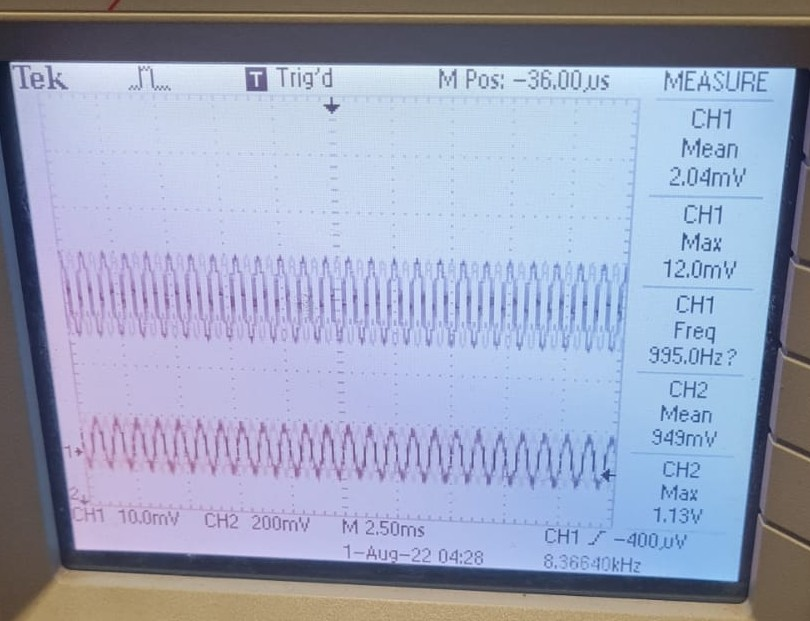
\includegraphics[width=0.7\linewidth]{currentSensor_impl_noise.jpeg}
      \captionof{figure}{Noise Level}
      \label{fig:results_currentSensor_noise}
   \end{minipage}
   \begin{minipage}{0.45\textwidth}
      \centering
      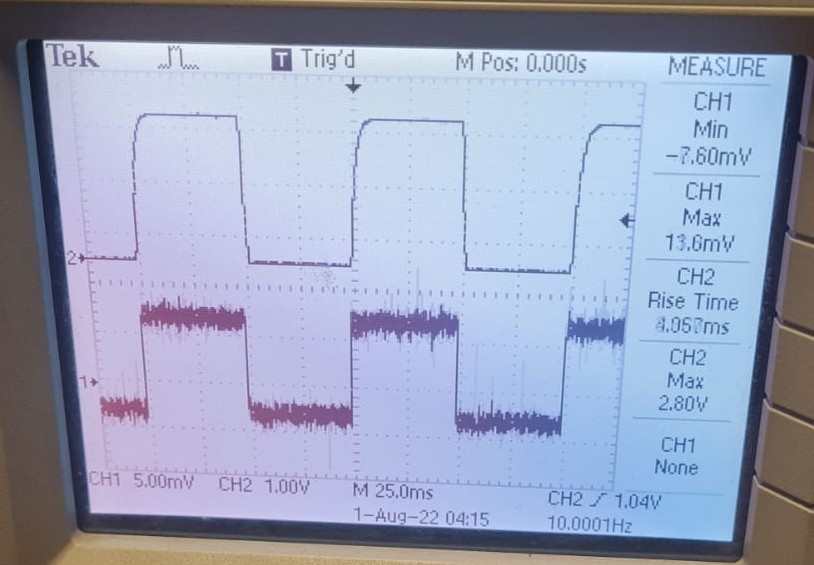
\includegraphics[width=0.7\linewidth]{currentSensor_impl_stepResponse.jpeg}
      \captionof{figure}{Step Response}
      \label{fig:results_currentSensor_response}
   \end{minipage}
\end{figure}

Current measurements were then made with the motor connected, as visible in Table \ref{table:motor_currents}.
As can be analyzed, there is an offset voltage of \SI{0.42}{V} at the output. The actual gain can be calculated as e.g.
$\frac{\SI{1.42}{V} - \SI{0.42}{V}}{\SI{210}{\milli\ampere} * \SI{10}{\milli\ohm}}= 476 V/V$. With the \SI{120}{\kilo\ohm} resistor,
an ideal gain of $\frac{\SI{120}{\kilo\ohm}}{\SI{330}{\ohm}} = 363.6V/V$ was expected, however due to the nature of the circuit
(which contains 4 resistors) a tolerance of 10\% * 4 should be accounted for, which explains the higher gain.

\begin{table}[!h]
   \centering
   \begin{tabular}{ |c|c|c| }
      \hline
      \textbf{Motor Condition}         & \textbf{PSU Current (mA)}        & \textbf{Output  Voltage (V)}       \\ \hline
      Stall                            & 1200                             & 3.31                               \\ \hline
      Slight Load                      & 305                              & 1.96                               \\ \hline
      Free Running                     & 210                              & 1.42                               \\ \hline
      I = 150 mA                       & 150                              & 1.13                               \\ \hline
      I = 100 mA                       & 100                              & 0.91                               \\ \hline
      I = 50 mA                        & 50                               & 0.63                               \\ \hline
      I = 0 mA                         & 0                                & 0.42                               \\ \hline
   \end{tabular}\
   \caption{Measurements of Motor Current and Voltage}
   \label{table:motor_currents}   
\end{table}

\begin{figure}[!h]
   \centering
   \begin{minipage}{0.3\textwidth}
      \centering
      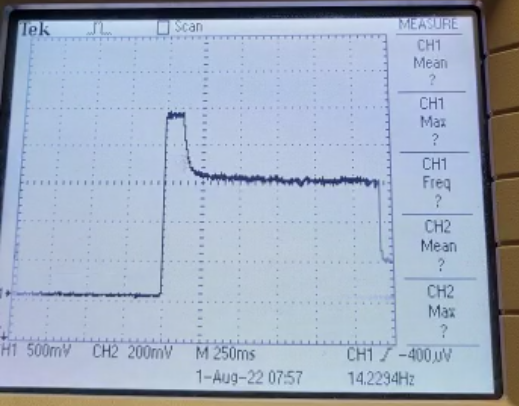
\includegraphics[width=0.7\linewidth]{currentSensor_impl_freeRunning}
      \captionof{figure}{Open Circuit to Free Running}
   \end{minipage}
   \begin{minipage}{0.3\textwidth}
      \centering
      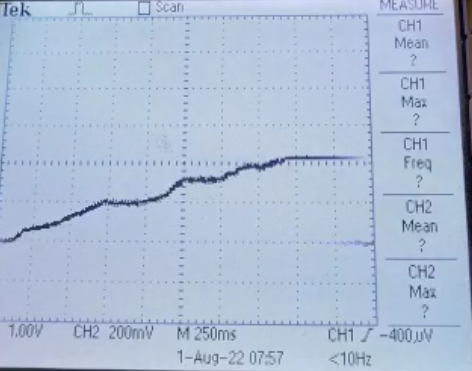
\includegraphics[width=0.7\linewidth]{currentSensor_impl_increasingLoad}
      \captionof{figure}{Increasing Load}
   \end{minipage}
   \begin{minipage}{0.3\textwidth}
      \centering
      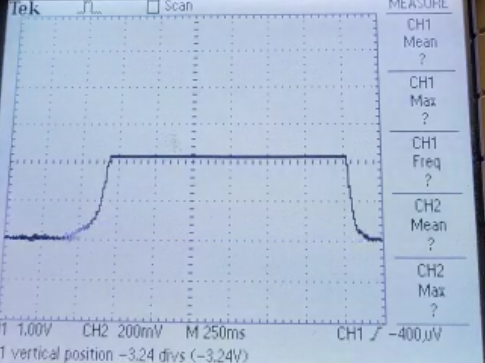
\includegraphics[width=0.7\linewidth]{currentSensor_impl_stall}
      \captionof{figure}{Free Running to Stall}
   \end{minipage}   
\end{figure}